\documentclass[12pt]{beamer}
\usepackage[utf8]{inputenc}
\usepackage[T1]{fontenc}
\usepackage{amsmath}
\usepackage{amsfonts}
\usepackage{amssymb}
\usepackage{graphicx}
\usepackage{bussproofs}
\usepackage{lmodern}
\newenvironment{boxedprooftree}[1][c]
 {\begin{tabular}[#1]{@{}c@{}}}
 {\DisplayProof\end{tabular}}
 
\usetheme{Copenhagen}
\usepackage{listings}

\lstdefinelanguage{JavaScript}{
  keywords={const, let, break, case, catch, continue, debugger, default, delete, do, else, finally, for, function, if, in, instanceof, new, return, switch, this, throw, try, typeof, var, void, while, with, class, constructor, public, private, boolean, string, number, export,yield, any},
  morecomment=[l]{//},
  morecomment=[s]{/*}{*/},
  morestring=[b]',
  morestring=[b]",
  sensitive=true
}

\lstset{
   language=JavaScript,
   showstringspaces=false,
   basicstyle=\tiny,
   showspaces=false,
   tabsize=2,
   escapechar={^}
}
\AtBeginSection[]
{
  \begin{frame}
    \frametitle{Table of Contents}
    \tableofcontents[currentsection]
  \end{frame}
}
\begin{document}
\newcommand{\mathsc}[1]{{\normalfont\textsc{#1}}}
%\newcommand{thunk}[2]{\mathbb{T}\left(#1,#2\right)}
\author{Ian Duncan and Ahmed Jellouli}
\title{Lazy Evaluation for Source}
%\subtitle{}
%\logo{}
%\institute{}
\date{CS4215 Final Project, 13 April 2020}
%\subject{Hi}
%\setbeamercovered{transparent}
\setbeamertemplate{navigation symbols}{}
\begin{frame}[plain]
	\maketitle
\end{frame}

\begin{frame}
\frametitle{Table of Contents}
\tableofcontents
\end{frame}

\section{Introduction}

\begin{frame}
\frametitle{Evaluation Strategies}
\begin{itemize}
\item<1->In \textbf{call-by-value} or \textbf{strict} evaluation, all arguments to a function are evaluated at application time.

\item<2->In \textbf{call-by-name} evaluation, arguments to a function are evaluated each time they are needed.

\item<3->In \textbf{call-by-need} or \textbf{lazy} evaluation, arguments to a function are evaluated the first time they are needed. The result of this evaluation is memoized in case the argument is needed again.
\end{itemize}
\end{frame}

\begin{frame}
\frametitle{Project Goals}
We aimed to produce a lazy version of Source\S2, which entailed the following deliverables:\pause
\begin{enumerate}
\item<2->A specification for ``Lazy Source'' 
\item<3->A metacircular evaluator
\item<4->Support for lazy evaluation in the interpreter and transpiler of \texttt{js-slang}
\item<5->Integration into Source Academy frontend
\item<5->Example programs
\item<7->Documentation
\end{enumerate}
\end{frame}

\section{Specification}

\begin{frame}
\frametitle{Inspiration}
Our specification follows the presentation of lazy evaluation in SICPJS\S4.2:\pause[1]
\begin{itemize}
\item<2->Application of user-defined functions is non-strict
\item<3->Application of built-ins (except for \texttt{pair} to support lazy lists), including binary operators is strict
\item<4->Evaluation of name bindings is strict
\end{itemize}
\pause[5]Note that this specification differs from Haskell, where \textit{all} of these are non-strict.
\end{frame}

\begin{frame}
\frametitle{Denotational Semantics of Source\S2}
In Source\S2, all function applications are strict:
\[
\begin{tabular}{@{} l c @{}}
[\textsc{App}] &
  \begin{boxedprooftree}
  \AxiomC{$\Delta\Vdash E_1\rightarrowtail f$}
  \AxiomC{$\Delta\Vdash E_2\rightarrowtail v_2,\ldots,\Delta\Vdash E_n\rightarrowtail v_n$}
  \BinaryInfC{$\Delta\Vdash E_1(E_2,\ldots,E_n)\rightarrowtail f(v_2,\ldots,v_n)$}
  \end{boxedprooftree}
\end{tabular}
\]
\end{frame}

\begin{frame}
\frametitle{Denotational Semantics of Delayed Computations}
\begin{itemize}
\item<1-> We introduce the concept of a \textbf{thunk}, which is an unevaluated expression and its associated environment, to support delayed evaluation of arguments.
\item<2-> In our denotation semantics, given an expression $E$ and associated environment $\Delta$, we represent the thunk of $E$ and $\Delta$ as $\theta(E, \Delta)$.
\item<3-> Thunks can be \textbf{forced} as needed:
\[
\begin{tabular}{@{} l c @{}}
[\textsc{Force}] &
  \begin{boxedprooftree}
  \AxiomC{$\Delta_1\Vdash E \rightarrowtail v$}
  \AxiomC{}
  \BinaryInfC{$\Delta_2\Vdash\theta(E, \Delta_1)\rightarrowtail v$}
  \end{boxedprooftree}
\end{tabular}
\]
\end{itemize}

\end{frame}

\begin{frame}
\frametitle{Denotational Semantics of Lazy Application}
In Lazy Source, we say that a function $f$ is \textbf{strict} if it is built-in (except for \texttt{pair}), and \textbf{non-strict} otherwise.\pause
\[
\begin{tabular}{@{} l c @{}}
[\textsc{SApp}] &
  \begin{boxedprooftree}
  \AxiomC{$\Delta\Vdash E_1\rightarrowtail f$}
  \AxiomC{$\Delta\Vdash E_2\rightarrowtail v_2,\ldots,\Delta\Vdash E_n\rightarrowtail v_n$}
  \BinaryInfC{$\Delta\Vdash E_1(E_2,\ldots,E_n)\rightarrowtail f(v_2,\ldots,v_n)$}
  \end{boxedprooftree}
\end{tabular}
\]
where $f$ is \textbf{strict}.\pause
\[
\begin{tabular}{@{} l c @{}}
[\textsc{NSApp}] &
  \begin{boxedprooftree}
  \AxiomC{$\Delta\Vdash E_1\rightarrowtail f$}
  \AxiomC{$E_2,\ldots,E_n$}
  \BinaryInfC{$\Delta\Vdash E_1(E_2,\ldots,E_n)\rightarrowtail f(\theta(E_2,\Delta),\ldots,\theta(E_n,\Delta))$}
  \end{boxedprooftree}
\end{tabular}
\]
where $f$ is \textbf{non-strict}.
\end{frame}
\section{Metacircular Evaluator}
\begin{frame}[fragile]
\frametitle{Representing Thunks}
We represent thunks as tagged lists:
\begin{lstlisting}[language=JavaScript]
function delay_it(exp, env) {
    return list("thunk", exp, env);
}

function thunk_exp(thunk) {
    return head(tail(thunk));
}

function thunk_env(thunk) {
    return head(tail(tail(thunk)));
}
\end{lstlisting}
\end{frame}

\begin{frame}[fragile]
\frametitle{Forcing Thunks}
To get the actual value of evaluating an expression (i.e., not a thunk), we define an \texttt{actual\_value} function:
\begin{lstlisting}
function actual_value(exp, env) {
    return force_it(evaluate(exp, env));
}
\end{lstlisting}
\end{frame}

\begin{frame}[fragile]
\frametitle{Forcing Thunks}
The function \texttt{force\_it} is mutually recursive with \texttt{actual\_value}, and handles memoization:
\begin{lstlisting}
function force_it(obj) {
    if(is_thunk(obj)) {        
        const result = actual_value(thunk_exp(obj), thunk_env(obj));        
        set_head(obj, "evaluated_thunk");
        set_head(tail(obj), result);
        set_tail(tail(obj), null);        
        return result;        
    } else if(is_evaluated_thunk(obj)) {        
        return thunk_value(obj);        
    } else {
        return obj;
    }    
}
\end{lstlisting}
\end{frame}

\begin{frame}[fragile]
\frametitle{Function Application}
We define two functions to help us delay or force function arguments as needed:
\begin{lstlisting}
function list_of_arg_values(exps, env) {
    return no_operands(exps)
        ? null
        : pair(actual_value(first_operand(exps), env),
          list_of_arg_values(rest_operands(exps), env));
}

function list_of_delayed_args(exps, env) {
    return no_operands(exps)
        ? null
        : pair(delay_it(first_operand(exps), env),
          list_of_delayed_args(rest_operands(exps), env));
}
\end{lstlisting}
\end{frame}

\begin{frame}[fragile]
\frametitle{Function Application}
Then we modify \texttt{apply} to delay or force arguments as needed:
\begin{lstlisting}
function apply(fun, args, env) {
    if (is_primitive_function(fun)) {
      return apply_primitive_function(fun, list_of_arg_values(args,env));
   } else if (is_compound_function(fun)) {
      ...
      const delayed_args = list_of_delayed_args(args, env);
      const values = append(delayed_args, temp_values);			   
      const result =
         evaluate(body,
                  extend_environment(
                      names,
                      values,
                      function_environment(fun)));
      ...
   }
   ...
}
\end{lstlisting}
\end{frame}

\begin{frame}[fragile]
\frametitle{Lazy Lists}
\end{frame}

\begin{frame}[fragile]
\frametitle{Evaluate}
Finally, we make a small change to the \texttt{evaluate} function to let \texttt{apply} have full control in handling function arguments. We also make sure the final result of evaluating a Source program is forced:
\begin{lstlisting}
function evaluate(stmt, env) {
   return is_self_evaluating(stmt)
          ?  stmt
        ...
        : is_application(stmt)
          ? is_pair_constructor(stmt) ? construct_lazy_pair(operands(stmt),env) 
           : apply(actual_value(operator(stmt), env),
                  operands(stmt), env)
        ...
}

function eval_toplevel(stmt) {
   const program_block = make_block(stmt);
   const value = actual_value(program_block, 
                          the_global_environment);
   ...
}
\end{lstlisting}
\end{frame}

\section{Implementation in \texttt{js-slang}}

\subsection{Overview}

\begin{frame}
\frametitle{Overview}
\begin{itemize}
\item<1-> We modify the interpreter and transpiler of \texttt{js-slang} to support lazy evaluation, if explicitly enabled.
\item<2-> The evaluation method (strict or lazy) is controlled by a \texttt{variant} property of the execution context.
\item<3-> The implementation of the interpreter mirrors that of the metacircular evaluator.
\item<4-> We modify the transpiler to thunk arguments in transpiled code if lazy evaluation is enabled, and alter native runtime operators to handle thunks if they are present.
\end{itemize}
\end{frame}

\subsection{Transpiler}

\begin{frame}[fragile]
\frametitle{Representing Thunks in Transpiled Code}
\begin{itemize}
\item<1-> Delaying a computation $E$ is as simple as making $E$ the body of a nullary arrow function: \texttt{() => E}

\item<2-> Since we also want to memoize our thunks, we create an object instead:
\begin{lstlisting}
{isThunk: true, expr: () => E, memoizedValue: 0, isMemoized: false}
\end{lstlisting}
\end{itemize}
\end{frame}

\begin{frame}
\frametitle{Creating Thunks at Compile Time}
\begin{itemize}
\item<1-> Function calls in Source are wrapped with a call to the native runtime operator \texttt{callIfFuncAndRightArgs}. For example, \texttt{f(a, b, c)} is transformed to \texttt{callIfFuncAndRightArgs(f, lineno, colno, a, b, c)}.
\item<2-> If lazy evaluation is enabled, we also thunk the arguments during this transformation. So, \texttt{f(a, b, c)} is transformed to \texttt{callIfFuncAndRightArgs(f, lineno, colno, \{expr: () => a, ...\}, ...)}
\item<3-> We alter the transformation \texttt{transformReturnStatementsToAllowProperTailCalls} in a similar way.
\end{itemize}
\end{frame}

\begin{frame}[fragile]
\frametitle{Handling Thunks at Runtime}
We define a new native runtime operator \texttt{forceIt} to force thunks when needed:
\begin{lstlisting}
export function forceIt(val: any): any {
  if (val !== undefined && val !== null && val.isThunk === true) {
    if (val.isMemoized) {
      return val.memoizedValue
    }
    const evaluatedValue = forceIt(val.expr())
    val.isMemoized = true
    val.memoizedValue = evaluatedValue
    return evaluatedValue
  } else {
    return val
  }
}
\end{lstlisting}
\end{frame}

\begin{frame}[fragile]
\frametitle{Handling Thunks at Runtime}
We then modify \texttt{callIfFuncAndRightArgs} to force thunks when necessary:
\begin{lstlisting}
export function callIfFuncAndRightArgs(candidate: any, line: number, column: number, 
                ...args: any[])
{
  ...
  candidate = forceIt(candidate)
  if (typeof candidate === 'function') {
    if (candidate.transformedFunction === undefined) {
      try {
        const forcedArgs = args.map(forceIt)
        return candidate(...forcedArgs)
      } catch (error) {
        ...
      }
    } else {
      ...
      return candidate(...args)
    }
  } else {
    ...
  }
}
\end{lstlisting}
\end{frame}

\begin{frame}
\frametitle{Handling Thunks at Runtime}
\begin{itemize}
\item<1-> We also make sure to force thunks in the native runtime operators \texttt{boolOrErr}, \texttt{unaryOp}, and \texttt{binaryOp} using \texttt{forceIt}.
\item<2-> Finally, we apply \texttt{forceIt} to the last statement in the program so that the final result of program evaluation is not a thunk.
\end{itemize}
\end{frame}

\subsection{Lazy Lists}

\begin{frame}
\frametitle{Lazy Lists}
\end{frame}

\subsection{Testing}

\begin{frame}[fragile]
\frametitle{Testing}
\begin{itemize}
\item<1-> We implement unit tests to show that the interpreter and transpiler both follow our specification for lazy evaluation.
\item<2-> We test memoization of thunks by making explicit use of side-effects:
\begin{lstlisting}
let x = 1;
function incX() {
  x = x + 1;
  return x;
}
function square(n) {
  return n * n;
}
square(incX()); // should evaluate to 4
\end{lstlisting}
\end{itemize}
\end{frame}

\section{Source Academy Frontend}

\begin{frame}
\frametitle{Source Academy Frontend}
We build on the work of Anubhav and Arsalan to add lazy variants of Source\S1 and Source\S2 to Source Academy:
\begin{center}
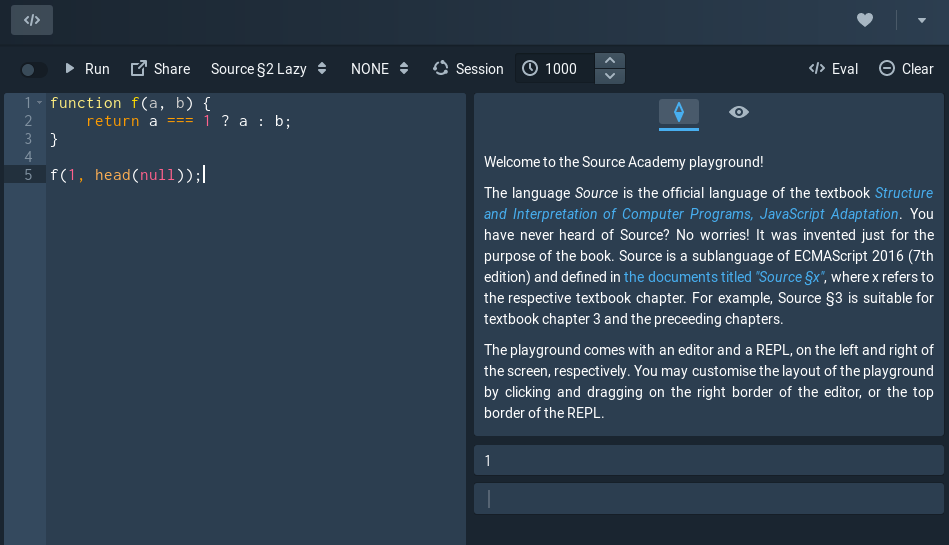
\includegraphics[width=0.7\linewidth]{safrontend}
\end{center}
\end{frame}

\section{Example Programs}

\subsection{The Power of Delayed Arguments}

\begin{frame}[fragile]
\frametitle{The Power of Delayed Arguments}
Consider the program:
\begin{lstlisting}
function f(a, b) {
	return a === 1 ? a : b;
}

f(1, head(null));
\end{lstlisting}\pause
Under strict evaluation, the call to \texttt{f} raises an error. However, under lazy evaluation \texttt{head(null)} is never evaluated because \texttt{b} is not used in \texttt{f} when \texttt{a} is 1, so no error is raised.
\end{frame}

\subsection{A List of all Factorial Numbers}

\begin{frame}
\frametitle{A Recursive Definition of Factorial}
Consider the following recursive definition of the factorial function:
\begin{align*}
0! &= 1 \\
(n+1)! &= (n+1)\times n!
\end{align*}
\end{frame}

\begin{frame}[fragile]
\frametitle{Combining Lists with \texttt{zipWith}}
We can combine the elements of two lists \texttt{xs} and \texttt{ys} into a single list with an additional function \texttt{f} using the operation \texttt{zipWith}:
\begin{lstlisting}
function zipWith(f, xs, ys) {
	return is_null(xs)
		? null
		: is_null(ys)
		? null
		: pair(f(head(xs), head(ys)), zipWith(f, tail(xs), tail(ys)))
}
\end{lstlisting}
\end{frame}

\begin{frame}[fragile]
\frametitle{A List of all Integers from $n$}
We can compute an infinite list of all integers from $n$:
\begin{lstlisting}
function intsFrom(n) {
	return pair(n, intsFrom(n+1));
}
\end{lstlisting}
\end{frame}

\begin{frame}[fragile]
\frametitle{Putting it all Together}
We can use \texttt{zipWith} and \texttt{intsFrom} to compute an infinite list of all factorials $0!, 1!, 2!,\ldots$:
\begin{lstlisting}
const factorials = pair(1, zipWith((x, y) => x*y, intsFrom(1), factorials));
\end{lstlisting}\pause
Conceptually, \texttt{factorials} is the list
\begin{align*}
1 &:: 1 \times 0! :: 2 \times 1! :: 3 \times 2! :: \cdots \\
0! &:: 1! :: 2! :: 3! :: \cdots
\end{align*}
To compute $n!$, just find the $n$th element of \texttt{factorials}.
\end{frame}

\end{document}